% ----------------
% 节: 附录A: SCU Theme 预览
% ----------------
\section{附录A: SCU Theme 预览}
\subsection{SCU Theme 选项预览}
\begin{frame}{Info.}
	\textbf{本小节将展示部分 SCU 主题选项的预览效果.}
	\begin{multicols}{2}
		\begin{itemize}
			\item \myestablish{v1.3e}{2024/10/31}
			\item \myupdate{v1.3e}{2024/10/31}
			\item \myupdate{v2.1b}{2025/10/06}
		\end{itemize}
	\end{multicols}
	注: 本小节仅对部分主题参数进行了演示, 您可点击标题栏 \texttt{BACK} 字样返回对应的宏包参数说明处.\par
	\mycopyright
\end{frame}

\begin{frame}{颜色主题预览 \scugoback{back:ColorDisplay}{BACK}}\label{goto:ColorDisplay}
  \structure{\cmd{usetheme}\oarg*{ColorDisplay=\Arg{value}}\marg*{scu}}
	\begin{columns}[T, onlytextwidth]
    \begin{column}{.5\textwidth}
      \structure{锦锈红} \Arg{value}\texttt{=JXred}
      \begin{figure}[h]
        \centering
        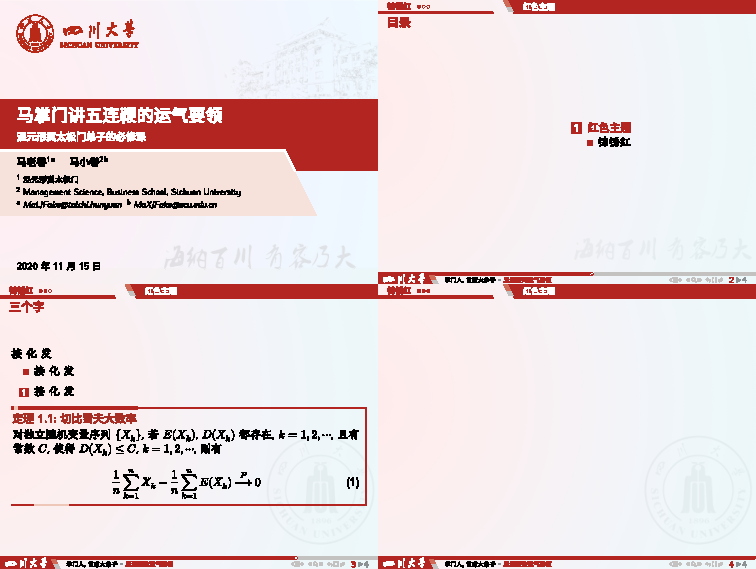
\includegraphics[width=\columnwidth]{manual-sec/manual-demo/appendix-themescu-ColorDisplay-1.pdf}
      \end{figure}
    \end{column}
    \begin{column}{.5\textwidth}
      \structure{宝石蓝} \Arg{value}\texttt{=BSblue}
      \begin{figure}[h]
        \centering
        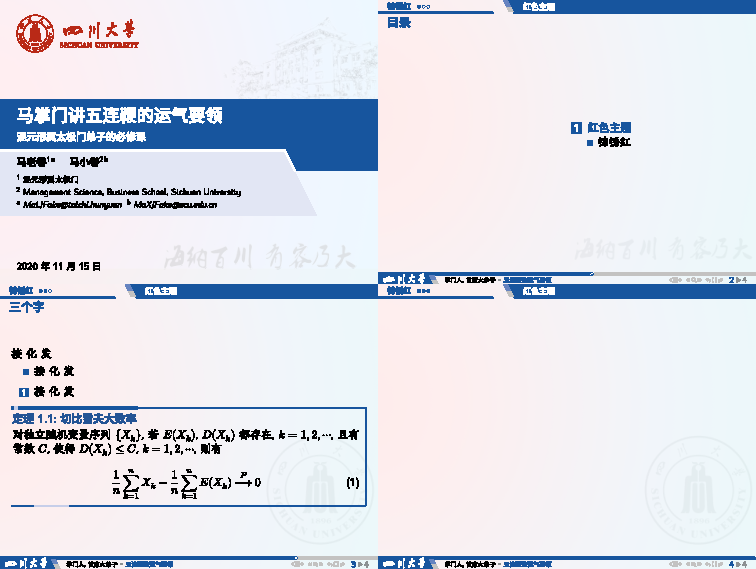
\includegraphics[width=\columnwidth]{manual-sec/manual-demo/appendix-themescu-ColorDisplay-2.pdf}
      \end{figure}
    \end{column}
  \end{columns}
\end{frame}

\begin{frame}{小节迷你帧预览 \scugoback{back:Miniframes}{BACK}}\label{goto:Miniframes}
  \vspace*{-6ex}
  \begin{figure}[h]
    \begin{tikzpicture}
      \node[anchor=south west] (img) at (0,10pt) {
\includegraphics[height=.88\textheight]{manual-sec/manual-demo/appendix-themescu-Miniframes.pdf}};
      \node[anchor=west] at (8, 211.4pt) {\structure{\cmd{usetheme}\oarg*{Miniframes=\Arg{value}}\marg*{scu}}};
      % --------- First ----------
      \def\xFir{28.8pt}
      \def\yFir{211.4pt}
      \draw[scublue, thin] (\xFir-6pt, \yFir-2pt) rectangle (\xFir+6pt, \yFir+2pt); % 以 (x, y) 为中心的框
      \draw[scublue, thin] (\xFir+6pt, \yFir-2pt) -- (\xFir+28pt, \yFir-13pt); % 斜线
      \draw[scublue, thin] (\xFir+28pt, \yFir-13pt) -- (8, \yFir-13pt); % 水平线
      \node[anchor=west] (NodeOne) at (8, \yFir-13pt) {\structure{迷你帧跟随} \Arg{value}\texttt{=follow}};
      \node[anchor=west] at ([yshift=-12pt]NodeOne.west) {迷你帧跟随当前小节标题(如此处为“小节迷你帧”)};
      % ---------- Second ----------
      \def\xSec{149.5pt}
      \def\ySec{154.2pt}
      \draw[scublue, thin] (\xSec-6pt, \ySec-2pt) rectangle (\xSec+6pt, \ySec+2pt); % 以 (x, y) 为中心的框
      \draw[scublue, thin] (\xSec+6pt, \ySec) -- (8, \ySec); % 水平线
      \node[anchor=west] (NodeTwo) at (8, \ySec) {\structure{迷你帧分离} \Arg{value}\texttt{=separate}};
      \node[anchor=west] at ([yshift=-12pt]NodeTwo.west) {迷你帧与小节标题分离(位于节导航栏下方且右侧对齐)};
      % ---------- Third ----------
      \def\xThiO{28.8pt}
      \def\yThiO{105.5pt}
      \draw[scublue, thin] (\xThiO-6pt, \yThiO-2pt) rectangle (\xThiO+6pt, \yThiO+2pt); % 以 (x, y) 为中心的框
      \draw[scublue, thin] (\xThiO+6pt, \yThiO-2pt) -- (\xThiO+28pt, \yThiO-13pt); % 斜线
      \draw[scublue, thin] (\xThiO+28pt, \yThiO-13pt) -- (8, \yThiO-13pt); % 水平线
      \def\xThiT{149.5pt}
      \def\yThiT{101.3pt}
      \draw[scublue, thin] (\xThiT-6pt, \yThiT-2pt) rectangle (\xThiT+6pt, \yThiT+2pt); % 以 (x, y) 为中心的框
      \draw[scublue, thin] (\xThiT+6pt, \yThiT-2pt) -- (\xThiT+19.6pt, \yThiT-8.8pt); % 斜线
      \node[anchor=west] (NodeThree) at (8, \yThiO-13pt) {\structure{取消迷你帧} \Arg{value}\texttt{=none}};
      \node[anchor=west] at ([yshift=-12pt]NodeThree.west) {页眉上无迷你帧显示};
      % ---------- Forth ----------
      \def\xForO{146.6pt}
      \def\yForO{48.2pt}
      \draw[scublue, thin] (\xForO-8pt, \yForO-2pt) rectangle (\xForO+8pt, \yForO+2pt); % 以 (x, y) 为中心的框
      \draw[scublue, thin] (\xForO+8pt, \yForO-2pt) -- (\xForO+20pt, \yForO-8pt); % 斜线
      \def\xForT{49pt}
      \def\yForT{31.4pt}
      \draw[scublue, thin] (\xForT-6pt, \yForT-2.8pt) rectangle (\xForT+6pt, \yForT+2.8pt); % 以 (x, y) 为中心的框
      \draw[scublue, thin] (\xForT+6pt, \yForT+2.8pt) -- (\xForT+18pt, \yForT+8.8pt); % 斜线
      \draw[scublue, thin] (\xForT+18pt, \yForT+8.8pt) -- (8, \yForT+8.8pt); % 水平线
      \node[anchor=west, align=left, yshift=-4pt] at (8, \yForT+8.8pt) {自v1.3e起, 迷你帧支持点击跳转\\若小节中页面数量过多且设置迷你帧跟随小节标题时\\\alert{迷你帧可自适应换行}\\反之设置迷你帧与小节标题分离则单行显示};
    \end{tikzpicture}
  \end{figure}
  \vspace*{-6ex}
\end{frame}

% ----------------
% 节: 附录B: SCU Theme 开发指南
% ----------------
\section{附录B: SCU Theme 开发指南}
\begin{frame}{序言}
	\textbf{SCU Theme 开发指南} (\textit{四川大学 Beamer 模板用户手册 - 附录B})旨在帮助
  \begin{itemize}
    \item \alert{他校师生}
    \item \alert{有个性化需求的使用者}
  \end{itemize}
  在现有 SCU Beamer Theme 基础上修改与扩展. 参照指南中主题结构、样式定义等说明, 您可根据自身需求灵活调整 Beamer 配色、版式和功能.\\

  在此希望这份开发指南不仅能作为四川大学 Beamer 模板的技术开发说明书, 也能成为一份可移植的参考文档, 供其他高校或研究团队在开发、定制 Beamer 主题时借鉴. 无论是为了匹配所需学术展示风格, 还是满足个人演示的个性化需求, 本指南都可为您提供清晰的实践思路.\\

  四川大学 Beamer 主题遵循 \alert{LaTeX Project Public License (LPPL)} 协议发布, 允许在保留署名的前提下自由修改与再分发. 同时, 也欢迎您反馈问题与改进建议, 以便不断完善和优化主题.\\

  \textbf{\alert{特别说明: 未经四川大学正式授权, 模板中涉及的校名、校徽等标志不得用于商业用途.}}
\end{frame}

\subsection{SCU Theme 项目结构}
\begin{frame}{Info.}
	\textbf{本小节将展示 SCU 主题的项目结构.}
	\begin{multicols}{2}
		\begin{itemize}
			\item \myestablish{v1.3e}{2024/10/31}
			\item \myupdate{v1.3e}{2024/10/31}
		\end{itemize}
	\end{multicols}
	注: 自 \textcolor{scugreen}{v1.3e (2024/10/31)} 起, 本小节已替代手册中\alert{\textbf{使用注意}}小节的\alert{项目结构}板块.\par
	\mycopyright
\end{frame}

\begin{frame}{\texttt{main} 分支文件结构 \scugoback{back:BranchMain}{BACK}}\label{goto:BranchMain}
  从 release 中下载的版本也具有如下的文件结构.
  \begin{multicols}{2}
    \setlength{\DTbaselineskip}{10pt}
    \dirtree{%
    .1 \alert{SCU Beamer Theme}/.
    .2 fonts/\DTcomment{\alert{字体存放}[资源]}.
    .2 image/\DTcomment{\alert{图像存放}[资源]}.
    .2 mintedbuild/\DTcomment{\alert{minted 缓存}[缓存]}.
    .2 resources/\DTcomment{\alert{\textbf{scu 主题素材}}[主题]}.
    .3 SCUbuilding.png\DTcomment{\text{建筑}[主题]}.
    .3 SCUlogo\_name.pdf\DTcomment{\text{logo + 校名}[主题]}.
    .3 SCUname.pdf\DTcomment{\text{校名}[主题]}.
    .3 SCUverify.png\DTcomment{\text{校训}[主题]}.
    .3 background.png.
    .3 backgroundofsubsectiontocpage.png.
    .3 backgroundoftitlepage(Empty).png.
    .3 backgroundoftitlepage(Light).png.
    .3 backgroundoftitlepage.png.
    .2 sourcecode/\DTcomment{\alert{代码存放}[资源]}.
    }
    \dirtree{%
    .1 \alert{SCU Beamer Theme}/.
    .2 beamercolorthemescu.sty\DTcomment{\alert{\textbf{颜色主题}}[主题]}.
    .2 beamerinnnerthemescu.sty\DTcomment{\alert{\textbf{内部主题}}[主题]}.
    .2 beamerouterthemescu.sty\DTcomment{\alert{\textbf{外部主题}}[主题]}.
    .2 beamerthemescu.sty\DTcomment{\alert{\textbf{scu核心主题}}[主题]}.
    .2 .gitignore.
    .2 LICENSE.
    .2 README.md.
    .2 main.tex\DTcomment{\alert{cn模式tex文件}[示例]}.
    .2 main.pdf\DTcomment{\alert{cn模式pdf文件}[示例]}.
    .2 main-en.tex\DTcomment{\alert{en模式tex文件}[示例]}.
    .2 main-en.pdf\DTcomment{\alert{en模式pdf文件}[示例]}.
    .2 manual.pdf\DTcomment{\alert{\textbf{用户手册}}[手册]}.
    .2 ref.bib\DTcomment{\alert{\textbf{文献库}}[资源]}.
    }
  \end{multicols}
\end{frame}

\begin{frame}{\texttt{manual} 分支文件结构 \scugoback{back:BranchManual}{BACK}}\label{goto:BranchManual}
  如下的示例演示资源中, pdf文件并不完全是tex直接编译所得, 而是编译后经过inkscape拼接、裁剪和压缩生成.
  \begin{multicols}{2}
    \setlength{\DTbaselineskip}{10pt}
    \dirtree{%
    .1 \alert{SCU Beamer Theme Manual}/.
    .2 manual-sec/\DTcomment{\alert{手册分节tex文件}[章节]}.
    .3 manual-demo/\DTcomment{\alert{手册中示例演示资源}[演示]}.
    .4 \text{...}.tex\DTcomment{\alert{示例tex文件}[演示]}.
    .4 \text{...}.pdf\DTcomment{\alert{示例pdf文件}[演示]}.
    .3 base-settings.tex\DTcomment{\alert{基础设置}[章节]}.
    .3 appendix-themescu.tex\DTcomment{\alert{附录}[章节]}.
    }\columnbreak
    \dirtree{%
    .1 \alert{SCU Beamer Theme Manual}/.
    .2 manual.tex\DTcomment{\alert{用户手册tex文件}[手册]}.
    .2 manual.pdf\DTcomment{\alert{用户手册pdf文件}[手册]}.
    }
  \end{multicols}
\end{frame}

\subsection{SCU Theme 主题自定义}
\begin{frame}{Info.}
	\textbf{本小节将给出 SCU Theme 的主题自定义实现方式.}
	\begin{multicols}{2}
		\begin{itemize}
			\item \myestablish{v2.1b}{2025/10/06}
		\end{itemize}
	\end{multicols}
	\mycopyright
\end{frame}

\begin{frame}{SCU Theme 颜色主题自定义(1/2) \scugoback{back:CustomColorTheme}{BACK}}\label{goto:CustomColorTheme}
	\structure{\cmd{usetheme}\oarg*{ColorDisplay=\Arg{value}}\marg*{scu}}

  当设置 \Arg{value} 为 \texttt{Custom} 时激活颜色主题自定义模式, 您可以参照如下步骤自定义颜色.\\

  \begin{columns}[T, onlytextwidth]
    \begin{column}{.67\textwidth}
      \structure{1. 在 \cmd{documentclass} 与 \cmd{usetheme} 间使用\\宏 \cmd{colorlet} 或 \cmd{definecolor} 定义下列颜色}\\

      \texttt{\% --- 如用 rgb 定义 ---}\\
      \cmd{definecolor}\marg*{PrimaryC}\marg*{rgb}\marg*{1,.41,.71}\texttt{\% 主题色-深粉}\\
      \cmd{definecolor}\marg*{NomalTextC}\marg*{rgb}\marg*{.2,.2,.2}\texttt{\% 普通文本-深灰}\\
      \cmd{definecolor}\marg*{AlertedTextC}\marg*{rgb}\marg*{1,.94,.96}\texttt{\% 强调文本-薰衣草紫红}\\
      \texttt{\% --- 如用 cmyk 定义 ---}\\
      \cmd{definecolor}\marg*{AuxiliaryC}\marg*{cmyk}\marg*{0,.25,0,0}\texttt{\% 辅助色-浅粉}\\
      \cmd{definecolor}\marg*{SecondaryAuxiliaryC}\marg*{cmyk}\marg*{0,.15,0,0}\texttt{\% 次级辅助色-更浅粉}\\
      \texttt{\% --- 如用 colorlet 派生/别名 ---}\\
      \cmd{colorlet}\marg*{BackgroundC}\marg*{white}\texttt{\% 背景主体-白色}\\
      \cmd{colorlet}\marg*{IntersperseC}\marg*{AuxiliaryC!50!PrimaryC}\texttt{\% 点缀色-粉色混合}\\
      \cmd{colorlet}\marg*{BlockExampleC}\marg*{AuxiliaryC!70!white}\texttt{\% 示例块-浅粉}\\
      \cmd{colorlet}\marg*{BlockLemmaC}\marg*{PrimaryC!60!white}\texttt{\% 引理块-淡粉}\\
      \cmd{colorlet}\marg*{BlockDefinitionC}\marg*{PrimaryC!80!black}\texttt{\% 定义块-深粉}\\
      \cmd{colorlet}\marg*{BlockConditionC}\marg*{AlertedTextC!50!white}\texttt{\% 条件块-淡紫红}\\
      \cmd{colorlet}\marg*{HighlightCodeLineC}\marg*{yellow!70!white}\texttt{\% 高亮代码行-浅黄}
    \end{column}
    \begin{column}{.33\textwidth}
      \structure{2. 在 \cmd{usetheme} 中设置选项}\\

      \cmd{usetheme}\oarg*{\%\\
        \hspace*{1em}ColorDisplay=Custom,\\
        \hspace*{1em}...\\
      }\marg*{scu}
    \end{column}
  \end{columns}
\end{frame}

\begin{frame}{SCU Theme 颜色主题自定义(2/2)}{深粉主题色预览}
\end{frame}


\begin{frame}{SCU Theme 字体主题自定义}
  定义微软雅黑字体 \cmd{setCJKsansfont}\oarg*{Scale=0.956}\marg*{Microsoft YaHei}\\

  定义思源黑体字体 \cmd{setCJKsansfont}\marg*{Noto Sans CJK SC}\\
\end{frame}

\begin{frame}{SCU Theme 背景及标识自定义}
  注:可使用以下方式临时修改背景及标识\\

  设置外部图片调用的代码如下: 

  \cmd{pgfdeclareimage}\oarg*{width=\Arg{value}, height=\Arg{value}}\texttt{\%}\\
    \hspace*{1em}\marg*{\Arg{image name}}\marg*{./resources/\Arg{image path}}\\

  \structure{修改封面页背景}
  
  定位到宏包文件 \pkg{beamethemescu.sty} 第 299 及 305 行, 修改图片 \texttt{bgoftitle} 对应的文件路径\\

  \structure{修改目录页背景}
  
  定位到宏包文件 \pkg{beamethemescu.sty} 第 293 行, 修改图片 \texttt{bgofsubsectoc} 对应的文件路径\\

  \structure{修改其他页背景}
  
  定位到宏包文件 \pkg{beamethemescu.sty} 第 288 行, 修改图片 \texttt{bg} 对应的文件路径\\

  \structure{修改 Logo, 带校名Logo, 建筑, 校训四个标识}

  定位到宏包文件 \pkg{beamethemescu.sty} 第 245 到 253 行, 分别修改图片 \texttt{lg}, \texttt{lg-name}, \texttt{building} 和 \texttt{verify} 对应的文件路径
\end{frame}

\begin{frame}{导航工具栏自定义 \scugoback{back:CustomNavigationTool}{BACK}}\label{goto:CustomNavigationTool}
  \structure{\cmd{usetheme}\oarg*{NavigationTool=\Arg{value}}\marg*{scu}}\vspace*{-2.5ex}
  \begin{figure}[h]
    \centering
    
\includegraphics[width=\textwidth]{manual-sec/manual-demo/appendix-themescu-NavigationTool.pdf}
  \end{figure}

  \structure{小节及小节跳转工具} 标记为1 - \alert{\hskip.4pt\setfontscu{5}\faCaretLeft\hskip1.6pt\faStream\hskip1.6pt\faCaretRight}\vspace*{1ex}

  \begin{tabular}{l>{\raggedright\arraybackslash}p{.02\textwidth}>{\raggedright\arraybackslash}p{.35\textwidth}l}
    核心工具 & {\setfontscu{5}\faStream} & 前往当前小节开始 & -\\
    附加工具 & {\setfontscu{5}\faCaretLeft} & 前往上一小节末尾 & -\\
    附加工具 & {\setfontscu{5}\faCaretRight} & 前往下一小节开始 & -\\
  \end{tabular}\vspace*{1ex}

  \structure{查询及首尾跳转工具} 标记为2 - \alert{\hskip.4pt\setfontscu{5}\faCaretLeft\hskip-.05em\faCaretLeft\hskip1.6pt\setfontscu{4.5}\faSearch\hskip1.6pt\setfontscu{5}\faCaretRight\hskip-.05em\faCaretRight}\vspace*{1ex}

  \begin{tabular}{l>{\raggedright\arraybackslash}p{.02\textwidth}>{\raggedright\arraybackslash}p{0.35\textwidth}l}
    核心工具 & {\setfontscu{4.5}\faSearch} & 查找(需要使用Adobe Acrobat) & Acrobat快捷键: Ctrl + F\\
    附加工具 & {\setfontscu{5}\faCaretLeft\hskip-.05em\faCaretLeft} & 前往初始页(不包含附录) & -\\
    附加工具 & {\setfontscu{5}\faCaretRight\hskip-.05em\faCaretRight} & 前往结尾页(不包含附录) & -\\
  \end{tabular}\vspace*{1ex}

  \structure{放映及历史跳转工具} 标记为3 - \alert{\hskip.4pt\setfontscu{4.5}\faReply\hskip1.6pt\setfontscu{5}\faExpand\hskip1.6pt\setfontscu{4.5}\reflectbox{\faReply}}\vspace*{1ex}

  \begin{tabular}{l>{\raggedright\arraybackslash}p{.02\textwidth}>{\raggedright\arraybackslash}p{0.35\textwidth}l}
    核心工具 & {\setfontscu{5}\faExpand} & 全屏或退出全屏(需要使用Adobe Acrobat) & Acrobat快捷键: Ctrl + L\\
    附加工具 & {\setfontscu{4.5}\faReply} & 前往上一视图(需要使用Adobe Acrobat) & Acrobat快捷键: Alt + 向左箭头\\
    附加工具 & {\setfontscu{4.5}\reflectbox{\faReply}} & 前往下一视图(需要使用Adobe Acrobat) & Acrobat快捷键: Alt + 向右箭头\\
  \end{tabular}
\end{frame}

%% End of file `appendix-themescu.tex'.